\section{Array-Based Data Structures} 

  What is the most simple type of data structure? In our daily lives, let's think of how we store data. 
  \begin{enumerate}
    \item A sentence consists of a sequence of words or letters. 
    \item A locker combination is a sequence of integers. 
    \item Accounting consists of logging a sequence of numbers for one's bank account. 
  \end{enumerate} 

  All of these things are sequential, so mathematically we can represent them as \href{st-def:sequence}{sequences}. However realistically we cannot have them be infinite like their mathematical analogue, so we work with arrays or lists.  

\subsection{Arrays and Lists} 

  The most simple form of a data structure requires us to fix a length $n$ of the number of elements it can contain. This is called an \textit{array}. 

  \begin{definition}[Array]
    An \textbf{array of size $n$} is a data structure $A$ that can contain up to $n$ elements in a specific order. The element in the $i$th index of $A$ is denoted $a_i$, and for most programming languages, we start at the index $i=0$, called \textbf{zero-indexing}.\footnote{When we say ``first,'' ``second,'' or ``third'' element in English, this will mean the elements on the $0$th, $1$st, and $2$nd index, respectively.} So our array would look like
    \begin{equation}
      A = [a_0, a_1, \ldots, a_n]
    \end{equation} 
    An uninitialized element will be denoted $a_i = \emptyset$. We also write $a_i = A[i]$. 
  \end{definition} 

  Great, so we have established our first data structure. Now we must be able to interact with it. The most elementary operations that we can do on $A$ is to add an element, remove an element, modify an element. Though this seems trivial at first glance, we must be careful on how the array is \textit{stored}. For example, if we store an array by writing down on a piece of paper, deleting an element (erasing it) would leave a whitespace gap where the original element was. We have to ask ourselves: are we fine with having this whitespace or should we shift the rest of the elements on the right one space to the left? Who even said that we have to shift the right-side elements? If we have deleted the second element, then we can just take the single element at index $0$ and shift that one right without having to move the rest of the list. 

  So there are a lot of nuances to this, and the efficiency of these operations really depend on how the arrays are stored. The question of how to store these lists efficiently will be thoroughly discussed in my architecture notes. 

  All these algorithms can be thought of as acting on an array $A$, denoted $\mathcal{A}(A)$. Let's go through them, starting with \textit{retrieval} of an element through a \textit{getter function}. 

  \begin{algo}[Retrieval of $i$th Element]
    Retrieval of the element $a_i$ at the $i$th index is $O(1)$.
    \begin{equation}
      [a_0, \ldots a_{i-1}, \emptyset, a_{i+1}, \ldots, a_{n-1}] \mapsto a_i 
    \end{equation}
  \end{algo}

  The next two---insert and modify---are called \textit{setter functions} since they set an element in array $A$ to a given value. 

  \begin{algo}[Insert Element to Array] 
    Insertion of element $b$ to index $i$ of array $A$ refers to replacing an uninitialized variable $a_i = \emptyset$ with $b$. This is $O(1)$. 
    \begin{equation}
      [a_0, \ldots a_{i-1}, \emptyset, a_{i+1}, \ldots, a_{n-1}] \mapsto [a_0, \ldots a_{i-1}, b, a_{i+1}, \ldots, a_{n-1}]
    \end{equation}
  \end{algo}
  
  \begin{algo}[Modify Element in Array]
    Modifying the $i$th element of array $A$ refers to replacing an initialized variable $a_i$ with an element $b$. This is $O(1)$. 
    \begin{equation}
      [a_1, \ldots a_{i-1}, a_i \neq \emptyset, a_{i+1}, \ldots, a_n] \mapsto [a_0, \ldots a_{i-1}, b, a_{i+1}, \ldots, a_{n-1}]
    \end{equation}
  \end{algo}

  \begin{algo}[Contains in Array]
    Given an element $b$, if we want to find out whether $b$ is contained in $A$, we must loop through the elements of $A$ and directly compare $b$ with $a_i$. This is $O(n)$. 
  \end{algo}

  \begin{algo}[Remove Element from Array]
    Removing the $i$th initialized element $a_i$ of array $A$ refers to deleting $a_i$, hence making it unitialized $a_i = \emptyset$. This is $O(1)$. 
    \begin{equation}
      [a_0, \ldots a_{i-1}, a_i, a_{i+1}, \ldots, a_{n-1}] \mapsto [a_0, \ldots a_{i-1}, \emptyset, a_{i+1}, \ldots, a_{n-1}]
    \end{equation}
  \end{algo} 

  Great, so we have achieved three constant-time methods to interact with this data structure. This is already quite intuitive, since inserting refers to writing a new record, modifying means overwriting a record, and removing means erasing a record. What else can we do? Inspired by our bookkeeping habits, we may want to talk about how many records we have in our array. 

  \begin{algo}[Size of Array]
    The size of an array can mean two things. 
    \begin{enumerate}
      \item If we want to talk about the number of elements it can store, it is $n$ by definition and thus getting this is $O(1)$. 
      \item If we want to find the number of initialized elements in $A$, then we must manually loop through the elements and see whether each $a_i$ is $\emptyset$ or not. This is $O(n)$. 
    \end{enumerate} 
  \end{algo} 

  While arrays are extremely useful, they may not be so flexible due to their rigid memory requirements. If we make an array of size 10 and find out later that we will need to store more than 10 elements, how should we proceed? An obvious solution is to just create a second array. But this requires us to keep track of multiple arrays for elements that are conceptually part of the same system, so this is untidy. A better alternative is to create a bigger array $B$, move all elements of the current array $A$ into $B$, and then just work with $B$. This motivates a \textit{list}.\footnote{Sometimes in literature, arrays and lists are used interchangeably. ArrayLists are also a term as well! However, in here, I will strictly differentiate arrays and lists.} 

  \begin{definition}[List]
    A \textbf{list} is a data structure $L$ that implements an array in the backend but a systematic way to dynamically grow in size. A list must have all of its elements initialized.\footnote{This also depends on the language/architecture, but we will follow Python's protocol.} The \textbf{size} of $L$ refers to the number of initialized elements in $L$.
    \begin{align}
      L & = [] \\
      L & = [1, 2, 3] \\
      L & = [a, c, b, l, p]
    \end{align}
  \end{definition} 

  Since the add operation depends on the growth of the list, we will introduce growth first. Clearly this growth 

  \begin{algo}[Grow Array Size of List]
    Given a list $L$ with an underlying array of length $n$, the grow operator 
    \begin{enumerate}
      \item first initializes a list $\hat{L}$ of size $f(n) > n$, and 
      \item second moves all elements from $L$ to $\hat{L}$, s.t. $\hat{L}[i] \gets L[i]$ for $i = 0, \ldots, n-1$. 
    \end{enumerate}
    For each $i$, getting $L[i]$ is $O(1)$ and setting $\hat{L}[i] \gets L[i]$ is also $O(1)$. Therefore by looping over $n$ elements this operation is $O(n)$. 
  \end{algo} 

  Clearly this growth operation is expensive, and we would like to do it a small number of times. A naive approach would be to start with a list of underlying array size $10$ and if we decide that we have to add, we can increase the size to $1,000, 000$. However, this may be wasteful in memory, especially if we later see that we need to store only $11$ elements. This is why a slightly more sophisticated growth scheme is preferred.

  \begin{example}[Some Growth Schemes]
    We present some growth schemes.
    \begin{enumerate}
      \item \textit{Increment by One}. The simplest approach is to increase the array size by 1 each time we need more space. When we have an array of size $n$ and need to add the $(n+1)$th element, we allocate a new array of size $n+1$, copy all $n$ elements, and add the new element. This gives sizes
      \begin{equation}
        1, 2, 3, 4, 5, \ldots, n
      \end{equation}
      While simple, this is inefficient as it requires $O(n^2)$ total copy operations to build a list of size $n$.

      \item \textit{Linear Growth}. We increase the array size by a constant factor $c$ each time. When we have an array of size $n$ and need more space, we allocate a new array of size $n+c$, where $c$ is some constant (e.g., $c=10$). This gives sizes
      \begin{equation}
        1, 1+c, 1+2c, 1+3c, \ldots, 1+kc
      \end{equation}
      This is better than increment by one, but still results in $O(n^2)$ total copy operations.

      \item \textit{Geometric Growth}. We start with a list of size $0$ (array size $1$). When we have an array size of $n$ and add the $n+1$th element, we increase the size of the array to $2n$. So our scheme gives sizes
      \begin{equation}
        1, 2, 4, 8, 16, \ldots
      \end{equation}
      This is how ArrayLists are implemented in Java. 

      \item \textit{Pseudo-Geometric Growth}.  Python uses a formula that increases the array size by approximately $1/8$ plus $3/4$ of the current size. When the list has size $n$, the new size becomes $|\hat{L}| = n + (n >> 3) + (n < 9 ? 3 : 6)$. This gives a sequence like
      \begin{equation}
        0, 4, 8, 16, 25, 35, 46, 58, 72, 88, \ldots
      \end{equation}
      which grows slightly slower than pure geometric growth but still maintains amortized $O(1)$ performance for appends.
    \end{enumerate}
  \end{example}

  This geometric growth is a good tradeoff between performance and memory usage. It never uses more than twice the memory of an array in order to store it. Furthermore, the runtime of a geometric growth pattern is amortized constant time, which means that it is constant when averaged over a long time. This is because the vast majority of these operations are constant time, with a few add operations which require resizing to be longer. But these few ones happen less and less frequently that when averaged over a long period, we can treat it as constant. 

  Now let's move onto the elementary operations of insert, delete, and modify. The fact that there can be no unitialized elements in our list means that there are extra nuances. 

  \begin{algo}[Retrieve ith Element from List]
    Retrieval of element $L[i]$ at index $i$ is $O(1)$. 
  \end{algo}

  \begin{algo}[Add Element to ith Index in List]
    Adding is a bit different. There are two cases. 
    \begin{enumerate}
      \item \textit{Adding to fixed index away from end}. If we do not have to grow the list, then we simply initialize the first open position with space this is $O(1)$. If we have to grow the list, this is $O(n)$.  
      \item \textit{Adding to any other index $i$}. If we have to grow the list, then we can add the elements $\hat{L}[j] \gets L[j]$ for $j < i$, then $\hat{L}[i] = b$, and then $\hat{L}[j+1] = L[j]$ for $j > i$. 
    \end{enumerate}

    Now assuming that we are using a geometric growth scheme (of $1, 2, 4, \ldots$), as we start with a list of size $0$ (array size $1$) and add $n$ elements to it, the total values copied is
    \begin{equation}
      1 + 2 + 4 + \ldots + (N/4) + (N/2) = N - 1
    \end{equation}
    Therefore, even though each growth is linear time, the frequency decays exponentially to the point that this is $O(n)$. Therefore, adding to the end of a list is \textit{on average} $O(1)$ time, also called \textit{amortized constant time}. 
  \end{algo}

  \begin{algo}[Modify ith Element in List]
    To modify $L[i]$ to a new value $b$ in a list, we can do this to the underlying array $A[i] \gets b$ in $O(1)$ time. 
  \end{algo}

  \begin{algo}[Contains in a List]
    Contains behaves the same as an array, with $O(n)$ time. 
  \end{algo} 

  \begin{algo}[Delete ith Element from List]
    Deleting also changes similarly to adding. 
    \begin{enumerate}
      \item \textit{Deleting to fixed index away from end}. We can delete it from the underlying array in $O(1)$ time, but this leaves $A[i] = \emptyset$. We must shift the rest of the rightmost elements to the left: $A[j] \gets A[j+1]$ for $i \leq j \leq n-1$. But since $j$ is a fixed index away from the end, we only have to most at most a constant number of elements $j$, so this is $O(j) = O(1)$
      \item \textit{Deleting to any other index $i$}. We have the same logic, but since $j$ is now not constant and can be any other index. Therefore in the worst case $j = 0$, and we must shift the entire array, leading to $O(n)$ runtime. 
      \item \textit{Deleting Index with Certain Value}. If we want to delete a certain value, we want to first scan the array to see if there contains an element with this value, and if so, we delete it. This gives $O(n)$ time.  
    \end{enumerate}
  \end{algo} 

  \begin{example}[String]
    The string type is just an ArrayList of characters. It has the following attributes and methods. Let $\texttt{x = "I love CS201"}$ 
    \begin{enumerate}
      \item $\texttt{int y = x.length()}$ outputs the length and is $O(1)$ 
      \item $\texttt{char y = x.charAt(0)}$ outputs a character and is $O(1)$
      \item $\texttt{String y = x.substring(0, 4)}$ 
      \item $\texttt{boolean y = x.equals("I love CS201")}$
      \item $\texttt{String y = x + "!!"}$ 
      \item $\texttt{String[] y = x.split(" ")}$
      \item $\texttt{String y = String.join(" ", words)}$
    \end{enumerate}
  \end{example} 

  While we could technically concatenate or reverse arrays, the presence of uninitialized elements make the algorithms implementation specific. We focus on lists. 

  \begin{algo}[Concatenating two Lists]
    
  \end{algo}

  \begin{algo}[Reversing List]
    $O(n)$
  \end{algo}

\subsection{Linked List and Iterators}

  \begin{definition}[Singly Linked List]
    A \textbf{singly linked list} contains a sequence of nodes that each contain an object for its element and a reference to the next node. More specifically, it can be divided up into 3 parts: 
    \begin{enumerate}
      \item The variable which points to the \textit{first} node. This can be confusing since this variable, which represents an \textit{entire list} is just a pointer to the first node. 
      \item A sequence of nodes containing the element and a reference to the next node. 
      \item The final node containing the element and a reference to $\texttt{null}$. 
    \end{enumerate}
    Unlike a list however, we will use \textbf{one-indexing} for linked lists, i.e. the head node is located at index $1$. 

    \begin{figure}[H]
      \centering 
      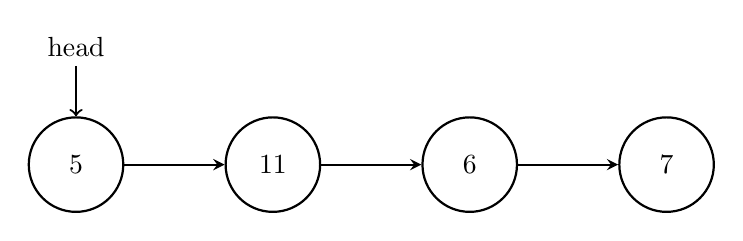
\begin{tikzpicture}[
            node/.style={circle, draw, minimum size=1.2cm, thick},
            arrow/.style={->, >=stealth, thick}
        ]

        % Nodes (circles)
        \node[node] (n1) at (0,0) {5};
        \node[node] (n2) at (2.5,0) {11};
        \node[node] (n3) at (5,0) {6};
        \node[node] (n4) at (7.5,0) {7};

        % Arrows connecting nodes
        \draw[arrow] (n1) -- (n2);
        \draw[arrow] (n2) -- (n3);
        \draw[arrow] (n3) -- (n4);

        % Head label and arrow
        \node[] (head) at (0,1.5) {head};
        \draw[->, black, thick] (head) -- (n1);
      \end{tikzpicture}
      \caption{The following diagram represents a linked list. But in reality, the elements are all located random in memory and can only be found by references. } 
      \label{fig:linked_list}
    \end{figure}
  \end{definition}

  \begin{algo}[Retrieve $i$th Element from Linked List]
    Given a linked list of size $n$ and some $1 \leq i \leq n$, retrieval of the $i$th value is $O(i)$, which 
    \begin{enumerate}
      \item in best case is $O(1)$ if $i$ is a fixed number not dependent on $n$. 
      \item in worst case is $O(n)$ if $i = n$, since we have to traverse through the $n-1$ nodes. 
    \end{enumerate}
  \end{algo}

  This is the first time we actually look at a nontrivial algorithm. 

  \begin{algo}[Insert Element to $i$th Index in Linked List]
    To add value $b$ as the $i$th element of a linked list, we must have first traverse through to the $i-1$ node $a_{i-1}$, then set it to point to $b$, and finally have $b$ point to $a_{i}$. The runtime is dominated by the first step of traversing, which is $O(i)$ and may be 
    \begin{enumerate}
      \item $\Theta(1)$ in the best case when $i=1$, or 
      \item $\Theta(n)$ in the worst case when $i=n$
    \end{enumerate}
    Note that this allows us to easily add to the beginning of a linked list, which was inefficient for regular lists. However, we now sacrifice the easy cost of adding to the end of the list, which worsened from $\Theta(1)$ to $\Theta(n)$. 

    \begin{algorithmic}[1]
      \Procedure{AddElementToLinkedList}{}
      % Variable initialization
      \State Linked list $L$, value $b$, index $i$ to insert to 
      \State $h, c \gets L$ \Comment{create references to head and current} 
      
      \For{$i \gets 1 \ldots i-2$} 
        \State $c \gets c.next$
      \EndFor 

      \State $t \gets c.next$  \Comment{Store temporary reference to $a_{i}$}
      \State $c.next \gets b$  \Comment{$a_{i}$ points to $b$}
      \State $b.next \gets t$  \Comment{$b$ points to $a_{i+1}$} 
      \State \Return{$h$} \Comment{return head}
      \EndProcedure
    \end{algorithmic}
  \end{algo}

  \begin{algo}[Modify $i$th Element in Linked List]
    Modifying is trivial since you just traversing the linked list to the $i$th node and then replace the value there. 
    \begin{enumerate}
      \item If $i$ is constant, then this is $\Theta(1)$. 
      \item If $i = n$ in the worst case, then this is $\Theta(n)$. 
    \end{enumerate}
  \end{algo}

  \begin{algo}[Contains in a Linked List]
    Checking containment just requires us to loop through all nodes and then determine whether our input value is equal to the value stored in the node. This requires us to loop through the entire list so is $\Theta(n)$. 
  \end{algo}

  \begin{algo}[Delete $i$th Element from Linked List]
    Deleting $a_i$ is the same logic as adding. We traverse the linked list until we get to node $a_{i-1}$, and then we set it to point to $a_{i+1}$. The runtime is dominated by the first step of traversing, which is $O(i)$ and may be 
    \begin{enumerate}
      \item $\Theta(1)$ in the best case when $i=1$, or 
      \item $\Theta(n)$ in the worst case when $i=n$
    \end{enumerate}

    \begin{algorithmic}[1]
      \Procedure{DeleteElementFromLinkedList}{}
      % Variable initialization
      \State Linked list $L$, index $i$ to insert to 
      \State $h, c \gets L$ \Comment{create references to head and current} 
      
      \For{$i \gets 1 \ldots i-2$} 
        \State $c \gets c.next$
      \EndFor 

      \State $c.next \gets c.next.next$ \Comment{Skip the next node and have it point to the node after}
      \State \Return{$h$} \Comment{return head}
      \EndProcedure
    \end{algorithmic}
  \end{algo} 

  \begin{algo}[Concatenating 2 Linked Lists]
    Given two linked lists $L_1, L_2$ of size $n, m$,  concatenating them to list $L_1 \oplus L_2$ is $O(n + m)$.
    \begin{algorithmic}[1]
      \Procedure{ConcatenateLinkedLists}{}
      \State Linked lists $L_1, L_2$
      \State $h_1, c_1 \gets L_1$ \Comment{create references to head and current of $L_1$} 
      
      \If{$h_1 = \text{null}$} \Comment{if $L_1$ is empty}
        \State \Return{$L_2$} \Comment{return $L_2$ as the result}
      \EndIf
      
      \While{$c_1.\text{next} \neq \text{null}$} \Comment{traverse to the end of $L_1$}
        \State $c_1 \gets c_1.\text{next}$
      \EndWhile
      
      \State $c_1.\text{next} \gets L_2$ \Comment{link the last node of $L_1$ to the head of $L_2$}
      
      \State \Return{$h_1$} \Comment{return the head of the concatenated list}
      \EndProcedure
    \end{algorithmic}
  \end{algo}

  \begin{algo}[Reversing a Linked List]
    Given a linked list $L$ of size $n$, reversing it has time complexity $O(n)$ as we need to traverse the entire list once. There is both an iterative and recursive approach. 
    
    \begin{algorithmic}[1]
      \Procedure{IterativeReverseLinkedList}{}
      \State Linked list $L$
      \State $prev \gets \text{null}$ \Comment{previous node, initially null}
      \State $curr \gets L$ \Comment{current node, starts at head}
      \State $next \gets \text{null}$ \Comment{to temporarily store the next node}
      
      \While{$curr \neq \text{null}$}
        \State $next \gets curr.\text{next}$ \Comment{store next node}
        \State $curr.\text{next} \gets prev$ \Comment{reverse the pointer}
        \State $prev \gets curr$ \Comment{move prev forward}
        \State $curr \gets next$ \Comment{move curr forward}
      \EndWhile
      
      \State \Return{$prev$} \Comment{prev is the new head of reversed list}
      \EndProcedure
    \end{algorithmic} 
    
    \begin{algorithmic}[1]
      \Procedure{RecursiveReverseLinkedList}{$head$}
      \If{$head = \text{null}$ or $head.\text{next} = \text{null}$}
        \State \Return{$head$} \Comment{Base case: empty list or single node}
      \EndIf
      
      \State $newHead \gets \Call{RecursiveReverseLinkedList}{head.\text{next}}$ \Comment{Reverse the rest}
      \State $head.\text{next}.\text{next} \gets head$ \Comment{Make next node point to current}
      \State $head.\text{next} \gets \text{null}$ \Comment{Remove original next pointer}
      
      \State \Return{$newHead$} \Comment{Return the new head (original tail)}
      \EndProcedure
    \end{algorithmic}
  \end{algo} 

  \begin{definition}[Doubly Linked List]
    A \textbf{doubly linked list} contains a sequence of nodes where each node contains an object for its element, a reference to the next node, and a reference to the previous node.
    \begin{enumerate}
      \item The variable which points to the 1st node is called the \textbf{head}. As with singly linked lists, this variable represents the \textit{entire list} but is just a pointer to the first node.
      \item A sequence of nodes, each containing the element, a reference to the next node, and a reference to the previous node.
      \item The final \textbf{tail} node containing the element, a reference to $\texttt{null}$ for its next pointer, and a reference to the second-to-last node for its previous pointer.
    \end{enumerate}
    Similar to singly linked lists, we will use \textbf{one-indexing} for doubly linked lists, i.e., the head node is located at index $1$.
    \begin{figure}[H]
      \centering 
      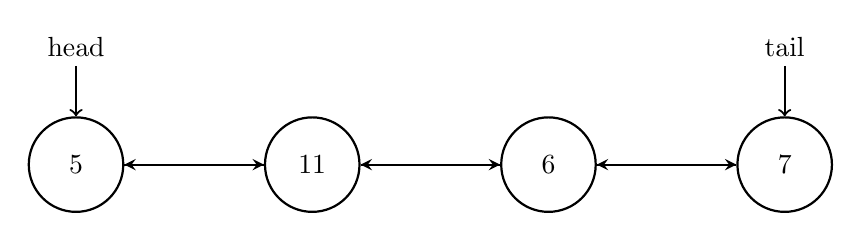
\begin{tikzpicture}[
            node/.style={circle, draw, minimum size=1.2cm, thick},
            arrow/.style={->, >=stealth, thick}
        ]
        % Nodes (circles)
        \node[node] (n1) at (0,0) {5};
        \node[node] (n2) at (3,0) {11};
        \node[node] (n3) at (6,0) {6};
        \node[node] (n4) at (9,0) {7};
        % Forward arrows connecting nodes
        \draw[arrow] (n1) -- (n2);
        \draw[arrow] (n2) -- (n3);
        \draw[arrow] (n3) -- (n4);
        % Backward arrows connecting nodes
        \draw[arrow] (n2) -- (n1);
        \draw[arrow] (n3) -- (n2);
        \draw[arrow] (n4) -- (n3);
        % Head label and arrow
        \node[] (head) at (0,1.5) {head};
        \draw[->, black, thick] (head) -- (n1);
        % Tail label and arrow (optional)
        \node[] (tail) at (9,1.5) {tail};
        \draw[->, black, thick] (tail) -- (n4);
      \end{tikzpicture}
      \caption{This diagram represents a doubly linked list. Forward pointers are shown in black, while backward pointers are shown in red. As with singly linked lists, the elements are located randomly in memory and can only be found through references. The presence of backward pointers allows for bidirectional traversal.}
      \label{fig:doubly_linked_list}
    \end{figure}
  \end{definition} 

  While we have to keep an extra pointer for every node in memory, this allows for simpler and sometimes more efficient implementations of the algorithms. For example, reversing a linked list can be done by simply swapping the previous and next pointers in each node. We can also add to and remove from both the front and back of a linked list in $O(1)$ time. 

  \begin{definition}[Circular Linked List]
    A \textbf{circular linked list} is a variation of a linked list where the last node, instead of pointing to null, contains a reference back to the first node, forming a circle or loop. This structure can be applied to both singly and doubly linked lists:
    \begin{enumerate}
      \item In a circular singly linked list, the last node's next pointer references the head node.
      \item In a circular doubly linked list, the last node's next pointer references the head node, and the head node's previous pointer references the last node.
    \end{enumerate}
    This circular nature allows traversal of the entire list starting from any node, as following the next pointers will eventually cycle through all nodes.
    \begin{figure}[H]
      \centering 
      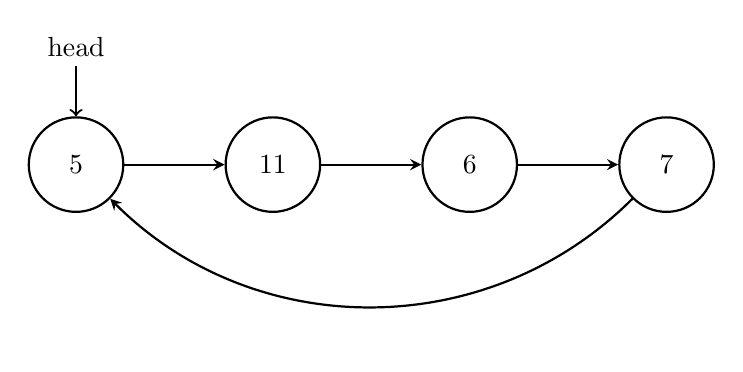
\begin{tikzpicture}[
            node/.style={circle, draw, minimum size=1.2cm, thick},
            arrow/.style={->, >=stealth, thick}
        ]
        % Nodes (circles)
        \node[node] (n1) at (0,0) {5};
        \node[node] (n2) at (2.5,0) {11};
        \node[node] (n3) at (5,0) {6};
        \node[node] (n4) at (7.5,0) {7};
        % Arrows connecting nodes (straight)
        \draw[arrow] (n1) -- (n2);
        \draw[arrow] (n2) -- (n3);
        \draw[arrow] (n3) -- (n4);
        % Circular connection
        \draw[arrow, bend left=45] (n4) to (n1);
        % Head label and arrow
        \node[] (head) at (0,1.5) {head};
        \draw[->, thick] (head) -- (n1);
      \end{tikzpicture}
      \caption{A circular singly linked list where the last node points back to the head node, creating a cycle. This structure eliminates the concept of a ``null end'' found in standard linked lists.}
      \label{fig:circular_linked_list}
    \end{figure}
  \end{definition}

  Let's introduce one more data structure. Note that even though our basic linked list solves the problem of adding in the beginning, in order to add in the middle or end, we must get to that position (which is $O(n)$ time) before we are able to utilize our $O(1)$ add. This is quite inefficient, especially when we do repeated adding, so we should keep track of certain "markers" that indicate where our current node is. \textit{Iterators} do this naturally, so we would like to implement some current notion of position. 

  \begin{definition}[Iterator]
    An \textbf{iterator} is a structure that maintains a reference a \textit{current position} within a list, along with methods to move the iterator to the next node (and previous node in doubly linked lists). 

    \begin{figure}[H]
      \centering 
      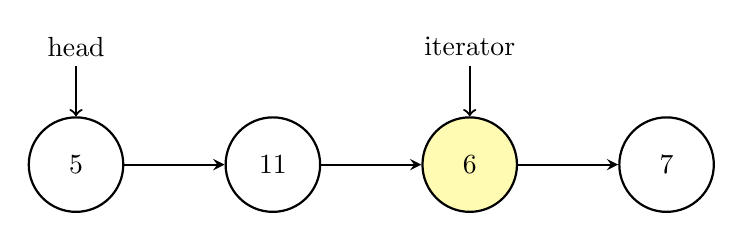
\begin{tikzpicture}[
            node/.style={circle, draw, minimum size=1.2cm, thick},
            arrow/.style={->, >=stealth, thick}
        ]
        % Nodes (circles)
        \node[node] (n1) at (0,0) {5};
        \node[node] (n2) at (2.5,0) {11};
        \node[node, fill=yellow!30] (n3) at (5,0) {6};
        \node[node] (n4) at (7.5,0) {7};
        % Arrows connecting nodes
        \draw[arrow] (n1) -- (n2);
        \draw[arrow] (n2) -- (n3);
        \draw[arrow] (n3) -- (n4);
        % Head label and arrow
        \node[] (head) at (0,1.5) {head};
        \draw[->, thick] (head) -- (n1);
        % Iterator label and arrow
        \node[] (iter) at (5,1.5) {iterator};
        \draw[->, thick] (iter) -- (n3);
      \end{tikzpicture}
      \caption{A linked list with an iterator currently positioned at the node containing the value 6. The iterator allows for immediate access to this position without traversing from the head.}
      \label{fig:linked_list_iterator}
    \end{figure}
  \end{definition}

  At first glance it may seem like iterators are just lists with less functionality, but we will see later that even non-array-like data structures can be turned into lists.  

\subsection{Stacks} 

  A stack is pretty much a list with a more limited set of operations, so whatever we can do with a stack we can do with a list. However, it is worth mentioning as its own data structure since it allows us to work with a simpler interface. 

  \begin{definition}[Stack]
    \label{def:stack}
    A \textbf{stack} is a data structure that stores data in the \textit{last-in-first-out (LIFO)} paradigm, which means that we can push (insert) elements into a stack $S$ and pop (remove) the last element that was pushed. 

    \begin{figure}[H]
      \centering 
      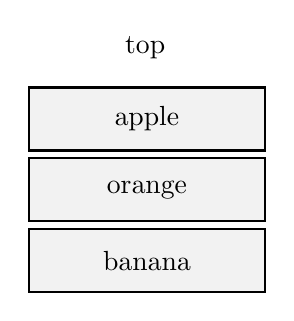
\begin{tikzpicture}[
        box/.style={rectangle, draw, thick, minimum width=3cm, minimum height=0.8cm, fill=gray!10}
        ]
        % Stack base
        \draw[thick] (0,0) -- (3,0);
        
        % Stacked items
        \node[box] (banana) at (1.5,0.4) {banana};
        \node[box] (orange) at (1.5,1.3) {orange};
        \node[box] (apple) at (1.5,2.2) {apple};
        
        \node[right] at (1.1,3.1) {top};
      \end{tikzpicture}
      \caption{We can literally imagine the elements of this list as ``stack.'' If you want to remove something from the stack, of course you have to remove the top element. } 
      \label{fig:stack}
    \end{figure}
  \end{definition} 

  The actual implementation can be done in many ways, either through a list or a linked list. 

  \begin{algo}[Push onto Stack]
    To push, i.e. add an element, onto the stack, we can 
    \begin{enumerate}
      \item insert to the end of a list, which is amortized $\Theta(1)$. 
      \item insert to the head of a singly linked list, which is $\Theta(1)$. 
    \end{enumerate}
  \end{algo}

  \begin{algo}[Pop from Stack]
    To pop, i.e. remove the last element pushed, from the (top of the) stack, we can 
    \begin{enumerate}
      \item remove the last element of a list, which is $\Theta(1)$. 
      \item move the head pointer to the second node and return the first node, which is $\Theta(1)$. 
    \end{enumerate}
  \end{algo}

  \begin{algo}[Peek into Stack]
    To peek, i.e. retrieve only the value at the top of the stack, we can 
    \begin{enumerate}
      \item return the last element of a list, which is $\Theta(1)$. 
      \item return the value of the head of the linked list, which is $\Theta(1)$. 
    \end{enumerate}
  \end{algo}

\subsection{Queues}

  \begin{definition}[Queue]
    A \textbf{queue} is an data structure that stores elements in the \textit{first-in-first-out (FIFO)} paradigm, which means that we can enqueue (insert) elements into a queue $Q$ and \textit{dequeue} (remove) elements in the order that they were pushed. 

    \begin{figure}[H]
      \centering 
      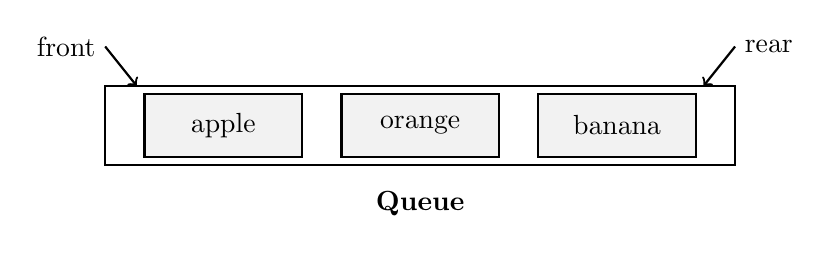
\begin{tikzpicture}[
        box/.style={rectangle, draw, thick, minimum width=2cm, minimum height=0.8cm, fill=gray!10}
        ]
        % Queue container
        \draw[thick] (0,0) rectangle (8,1);
        
        % Queue items
        \node[box] (apple) at (1.5,0.5) {apple};
        \node[box] (orange) at (4,0.5) {orange};
        \node[box] (banana) at (6.5,0.5) {banana};
        
        % Queue label
        \node[font=\bfseries] at (4,-0.5) {Queue};
        
        % Front and rear pointers
        \draw[->, thick] (0,1.5) -- (0.4,1);
        \node[left] at (0,1.5) {front};
        
        \draw[->, thick] (8,1.5) -- (7.6,1);
        \node[right] at (8,1.5) {rear};
      \end{tikzpicture}
      \caption{This is just like how a queue works. Whatever has been waiting in the queue the longest is the one that is removed first (at the front).} 
      \label{fig:queue}
    \end{figure}
  \end{definition} 

  Unlike a stack, which can be implemented with a list or linked list, for queues we must implement with a linked list with both a head and a tail pointer (or a doubly linked list). If we use a list, then to enqueue in $\Theta(1)$ time we must have it add to the end of the list, but when dequeuing, we must remove from the front of a list, which is inevitably $\Theta(n)$. The linked list has the opposite problem. Dequeuing is easy since we can shift the head node, but enqueuing requires us to traverse to the end before adding another node, which is $\Theta(n)$. In fact, Python implements this as a double ended queue.\footnote{\texttt{from collections import deque} where deque stands for double ended queue.} However, we will work with the minimal data structure of a singly linked list with a head and tail pointer. 

  \begin{algo}[Enqueue onto Queue]
    To enqueue an element $b$, we can have the tail pointer $a_n$ point to $b$ and update the tail pointer to $b$. This is $\Theta(1)$. 
  \end{algo}

  \begin{algo}[Dequeue onto Queue]
    To dequeue, we can return the head $a_1$ and update the head pointer to $a_2$.  
  \end{algo}

  \begin{algo}[Peek into Queue]
    To peek into the queue, we can simply return the value of the head pointer $a_1$. 
  \end{algo}

